\documentclass[12pt, a4paper, simple]{eskdtext}

\usepackage{hyperref}
\usepackage{env}
\usepackage{_sty/gpi_lst}
\usepackage{_sty/gpi_toc}
\usepackage{_sty/gpi_t}
\usepackage{_sty/gpi_p}
\usepackage{_sty/gpi_u}

% Код
% \ESKDletter{О}{Л}{Р}
% \def \gpiDocTypeNum {81}
% \def \gpiDocVer {00}
% \def \gpiCode {\ESKDtheLetterI\ESKDtheLetterII\ESKDtheLetterIII.\gpiStudentGroupName\gpiStudentGroupNum.\gpiStudentCard-0\gpiDocNum~\gpiDocTypeNum~\gpiDocVer}

\def \gpiDocTopic {Отчёт лабораторной работы №\gpiDocNum}

% колонтитулы
\usepackage{fancybox, fancyhdr}
\fancypagestyle{plain}
{
    \renewcommand{\footrulewidth}{0pt}          % Толщина отделяющей полоски снизу
    \renewcommand{\headrulewidth}{0pt}          % Толщина отделяющей полоски сверху
    \fancyhead[C]{ }                            % Коллонтитул сверху
    \fancyfoot[C]{\hfill\hfillстр. \thepage}    % Коллонтитул снизу
}

% Графа 1 (наименование изделия/документа)
% \ESKDcolumnI {\ESKDfontII \gpiTopic \\ \gpiDocTopic}

% Графа 2 (обозначение документа)
% \ESKDsignature {\gpiCode}

% Графа 9 (наименование или различительный индекс предприятия) задает команда
% \ESKDcolumnIX {\gpiDepartment}

% Графа 11 (фамилии лиц, подписывающих документ) задают команды
% \ESKDcolumnXIfI {\gpiStudentSurname}
% \ESKDcolumnXIfII {\gpiTeacherSurname}
% \ESKDcolumnXIfV {\gpiTeacherSurname}

\begin{document}
    \begin{ESKDtitlePage}
    \ESKDstyle{empty}
    \begin{center}
        \gpiMinEduRep \\
        \gpiEduRep \\
        \gpiKafRep \\
    \end{center}

    \vfill

    \begin{center}
        Тема: <<\gpiTopicRep>>
    \end{center}

    \vfill

    \begin{center}
        \textbf{\gpiDocTopic} \\
        по дисциплине \gpiDisciplineRep \\
    \end{center}

    \vfill

    \begin{flushright}
        \begin{minipage}[t]{7cm}
            Выполнил:\\
            \PageTitleStudentInfo
            \PageTitleDateField
            \hspace{0pt}

            Проверил:\\
            \PageTitleTeacherInfo
            \PageTitleDateField
        \end{minipage}
    \end{flushright}

    \vfill

    \begin{center}
        \PageTitleCity~\ESKDtheYear
    \end{center}
\end{ESKDtitlePage}

    \ESKDstyle{empty}
    \thispagestyle{plain}
    \pagestyle{plain}

    \begin{center}
        \textbf{\gpiDocTopic}
    \end{center}

    % = = = = = = = =
    \paragraph{} \textbf{Тема}: <<\gpiTopicRep>>

    \paragraph{} \textbf{Цель}:
    Формирование знаний и умений по разработке и оценке концепции АСОИ на основе требований заказчика.

    % \paragraph{} \textbf{Что нужно сделать}:

    % \paragraph{} \textbf{Разработка дизайна}:

    \paragraph{} \hspace{0pt}

    \begin{figure}[h!]
        \centering
        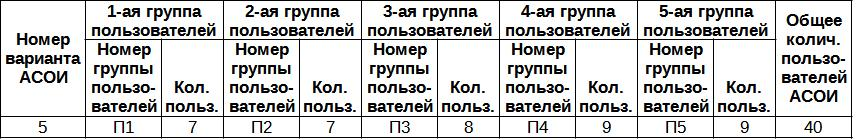
\includegraphics[width=16cm]
            {_docs/МоделиОрганизационнойСтруктурыОА.jpg}
        \caption{(Таблица В.1) Модели организационной структуры ОА}
    \end{figure}

    \begin{figure}[h!]
        \centering
        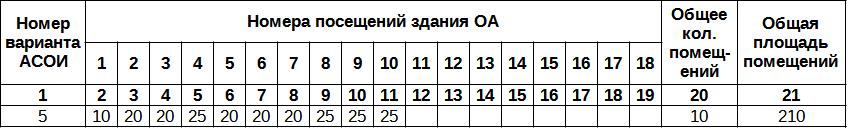
\includegraphics[width=16cm]
            {_docs/КаталогПомещенийЗданияИИхПлощадь.jpg}
        \caption{(Таблица В.2) Каталог помещений здания и их площадь}
    \end{figure}

    \begin{figure}[h!]
        \centering
        % \includegraphics[]
            % {_docs/ВариантыОбщейМоделиФункциональнойСтруктурыОА.jpg}
        \caption{(Рисунок Г.1) Варианты общей модели функциональной структуры ОА}
    \end{figure}

    \begin{figure}[h!]
        \centering
        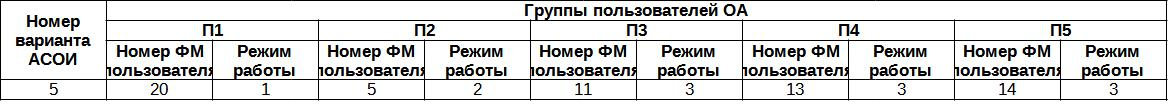
\includegraphics[width=16cm]
            {_docs/ВариантыРежимовРаботыГруппПользователейОА.jpg}
        \caption{(Таблица Г.1) Варианты режимов работы групп пользователей ОА}
    \end{figure}

    \begin{figure}[h!]
        \centering
        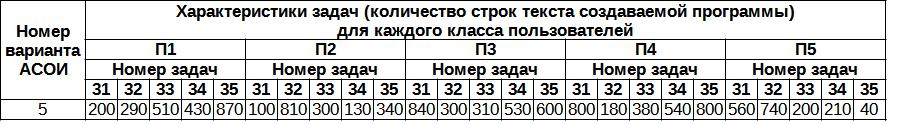
\includegraphics[width=16cm]
            {_docs/КаталогХарактеристикЗадачГруппПользователей.jpg}
        \caption{(Таблица Г.2) Каталог характеристик задач групп пользователей}
    \end{figure}

    \begin{figure}[ph!]
        \centering
        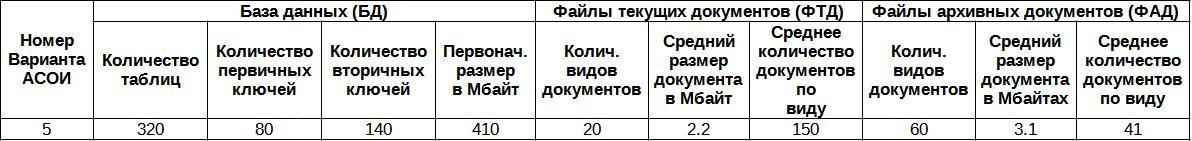
\includegraphics[width=16cm]
            {_docs/КаталогЭлементовИнформационнойСтруктурыОА.jpg}
        \caption{(Таблица Д.1) Каталог элементов информационной структуры ОА}
    \end{figure}

    \begin{figure}[ph!]
        \centering
        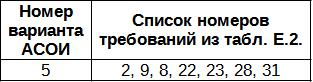
\includegraphics[]
            {_docs/ПереченьТребованийКСистемнымИИнструментальнымПрограммам.jpg}
        \caption{(Таблица Е.1) Перечень требований к системным и инструментальным программам}
    \end{figure}

    \begin{figure}[ph!]
        \centering
        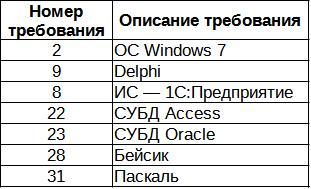
\includegraphics[]
            {_docs/КаталогТребованийКСистемнымИИнструментальнымПрограммам.jpg}
        \caption{(Таблица Е.2) Каталог требований к системным и инструментальным программам}
    \end{figure}

    \begin{figure}[ph!]
        \centering
        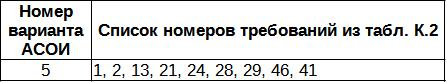
\includegraphics[]
            {_docs/ПереченьНомеровТребованийКТехническимСредствамАСОИ.jpg}
        \caption{(Таблица К.1) Перечень номеров требований к техническим средствам АСОИ}
    \end{figure}

    \begin{figure}[ph!]
        \centering
        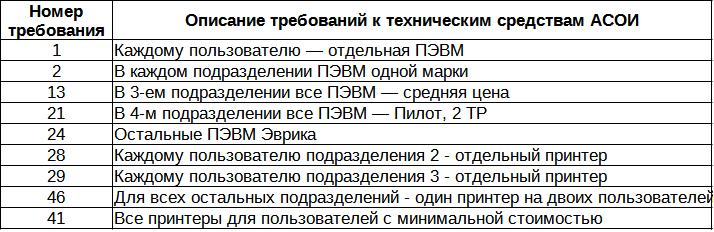
\includegraphics[]
            {_docs/КаталогТребованийКТехническимСредствамАСОИ.jpg}
        \caption{(Таблица К.2) Каталог требований к техническим средствам АСОИ}
    \end{figure}

    \begin{figure}[ph!]
        \centering
        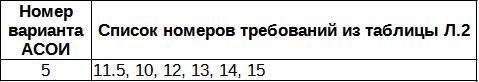
\includegraphics[]
            {_docs/СпискиНомеровТребованийКПроцессамЖЦАСОИ.jpg}
        \caption{(Таблица Л.1) Списки номеров требований к процессам ЖЦ АСОИ}
    \end{figure}

    \begin{figure}[ph!]
        \centering
        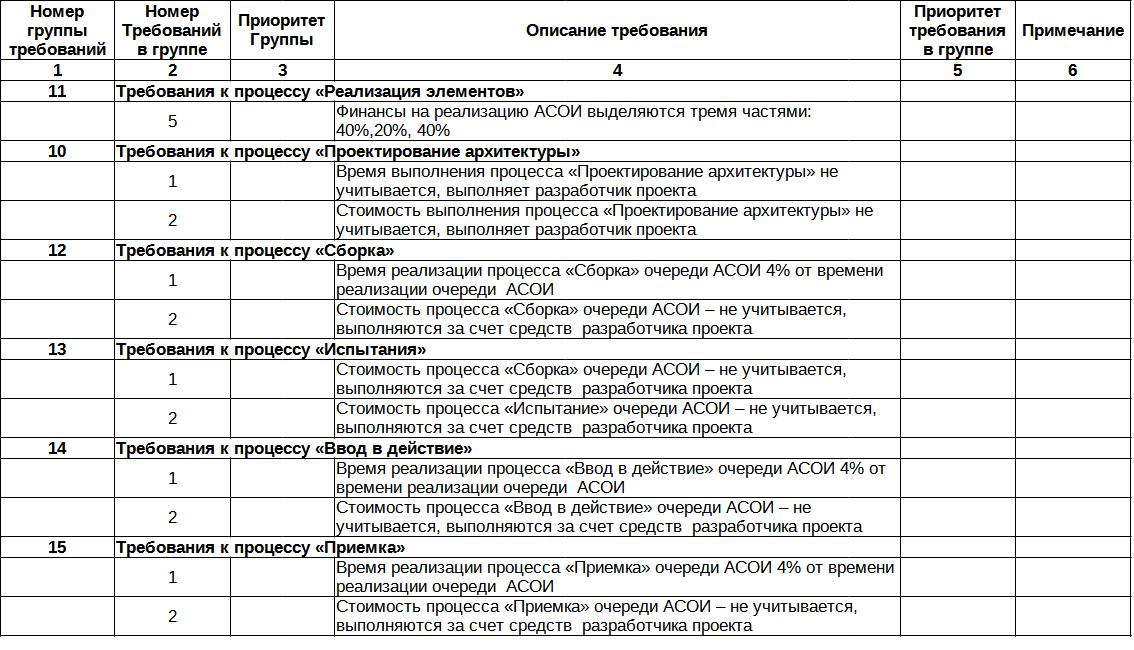
\includegraphics[width=16cm]
            {_docs/КаталогТребованийКПроцессамЖЦАСОИ.jpg}
        \caption{(Таблица Л.2) Каталог требований к процессам ЖЦ АСОИ}
    \end{figure}

    \begin{figure}[ph!]
        \centering
        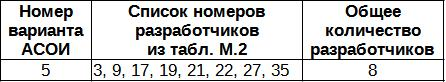
\includegraphics[]
            {_docs/СпискиНомеровРазработчиковЭлементовАСОИ.jpg}
        \caption{(Таблица М.1) Списки номеров разработчиков элементов АСОИ}
    \end{figure}

    \begin{figure}[ph!]
        \centering
        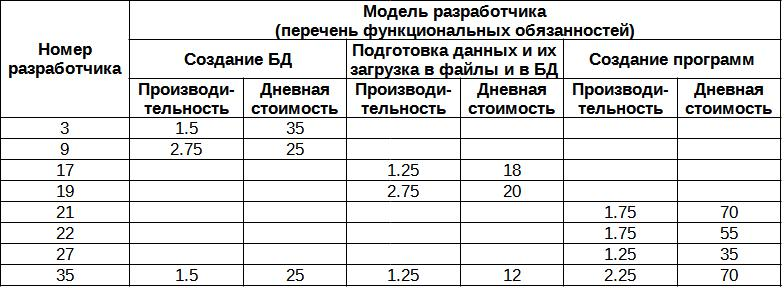
\includegraphics[width=16cm]
            {_docs/КаталогРазработчиковЭлементовАСОИ.jpg}
        \caption{(Таблица М.2) Каталог разработчиков элементов АСОИ}
    \end{figure}

    \newpage

    Так как все принтеры с минимальной стоимостью, то ищем минимальную стоимость принтера (Таблица Б.1 в общих требованиях).
    Минимальная стоимость 190.

    \begin{figure}[h!]
        \centering
        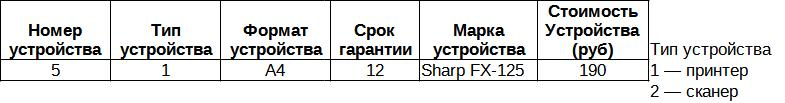
\includegraphics[width=16cm]
            {_docs/КаталогУстройств.jpg}
        \caption{(Таблица Б.1) Каталог устройств}
    \end{figure}

    3-ему подразделению ПЭВМ со средней ценой, а средняя цена по центру (Таблица Б.2 в общих требованиях).
    Средняя цена 505.

    4-ому подразделению ПЭВМ Пилот, 2 TP. Ищем в таблице (Таблица Б.2 в общих требованиях) марку ПЭВМ - пилот, внешнюю память - 2 Tb. 

    \begin{figure}[h!]
        \centering
        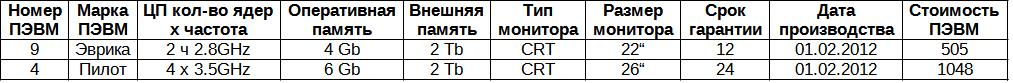
\includegraphics[width=16cm]
            {_docs/КаталогПЭВМ.jpg}
        \caption{(Таблица Б.2) Каталог ПЭВМ}
    \end{figure}

    Соотносим таблицу E.2 (индивидуальных требований варината 5) с таблицей Б.3 (общих требований).
    1) ОС Windows 7 - Windows7. 2) Delphi - Delphi, 3)  ИС-1С:Предприятие - 1С:Предприятие.
    4) СУБД Access - Access. 5) СУБД Oracle - Oracle. 6) Бейсик - нет. 7) Паскаль - нет. 

    \begin{figure}[h!]
        \centering
        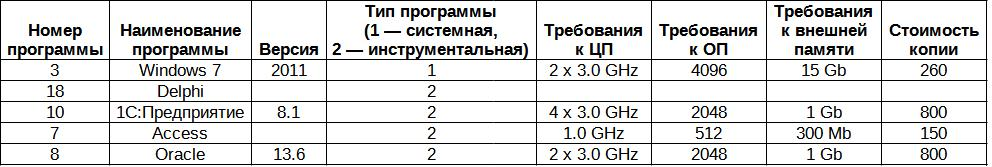
\includegraphics[width=16cm]
            {_docs/КаталогСистемныхИИнструментальныхПрограмм.jpg}
        \caption{(Таблица Б.3) Каталог системных и инструментальных программ}
    \end{figure}

    % \begin{sidewaysfigure}
    %     \centering
    %     \includegraphics[width=28cm]
    %         {_docs/КонцепцияАСИЕеКомпоненты.jpg}
    %     \caption{(Таблица 3.1) Концепция АС и её компоненты}
    % \end{sidewaysfigure}

    \newpage

    \begin{figure}[!hp]
        \centering
        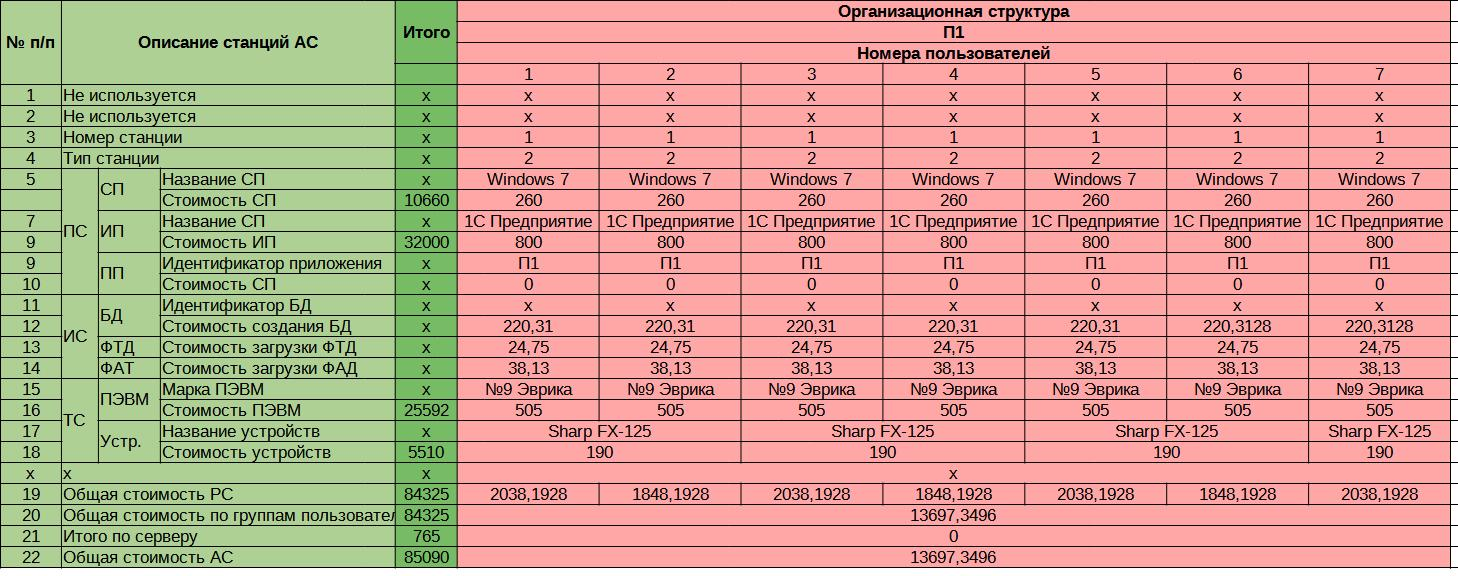
\includegraphics[height=6cm]
            {_docs/КонцепцияАСИЕеКомпонентыП1.jpg}
        \caption{(Таблица 3.1) Концепция АС и её компоненты}
    \end{figure}

    \begin{figure}[!hp]
        \centering
        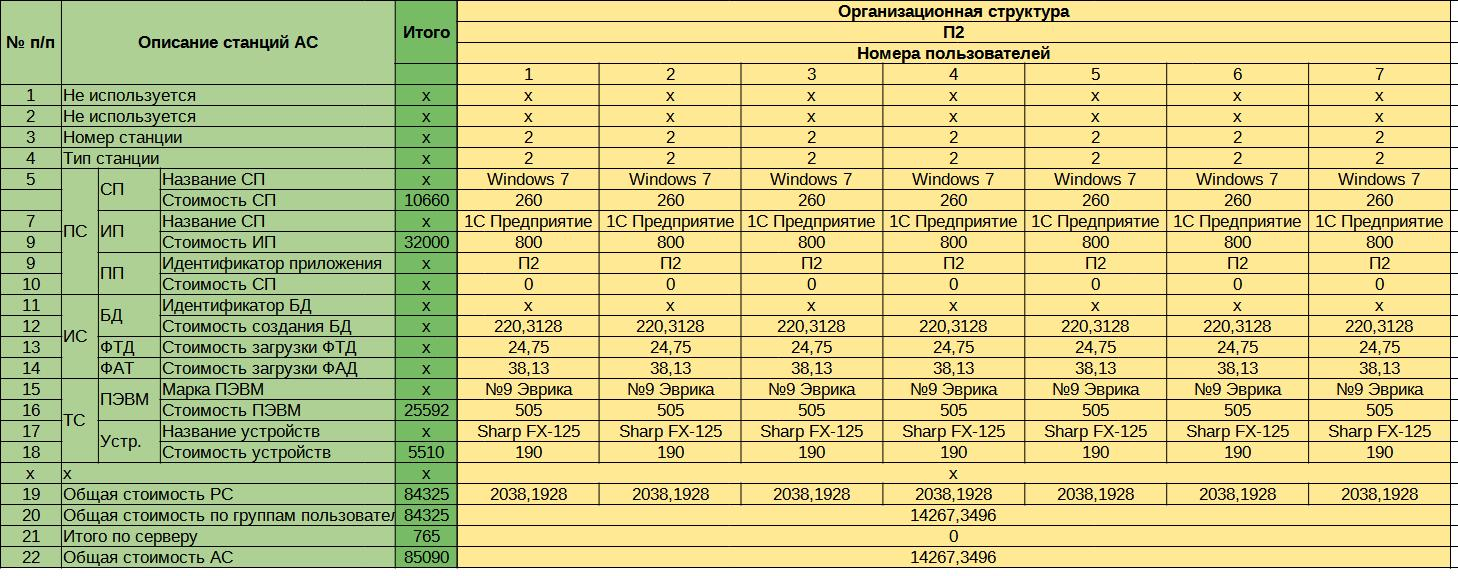
\includegraphics[height=6cm]
            {_docs/КонцепцияАСИЕеКомпонентыП2.jpg}
        \caption{(Таблица 3.1) Концепция АС и её компоненты}
    \end{figure}

    \begin{figure}[!hp]
        \centering
        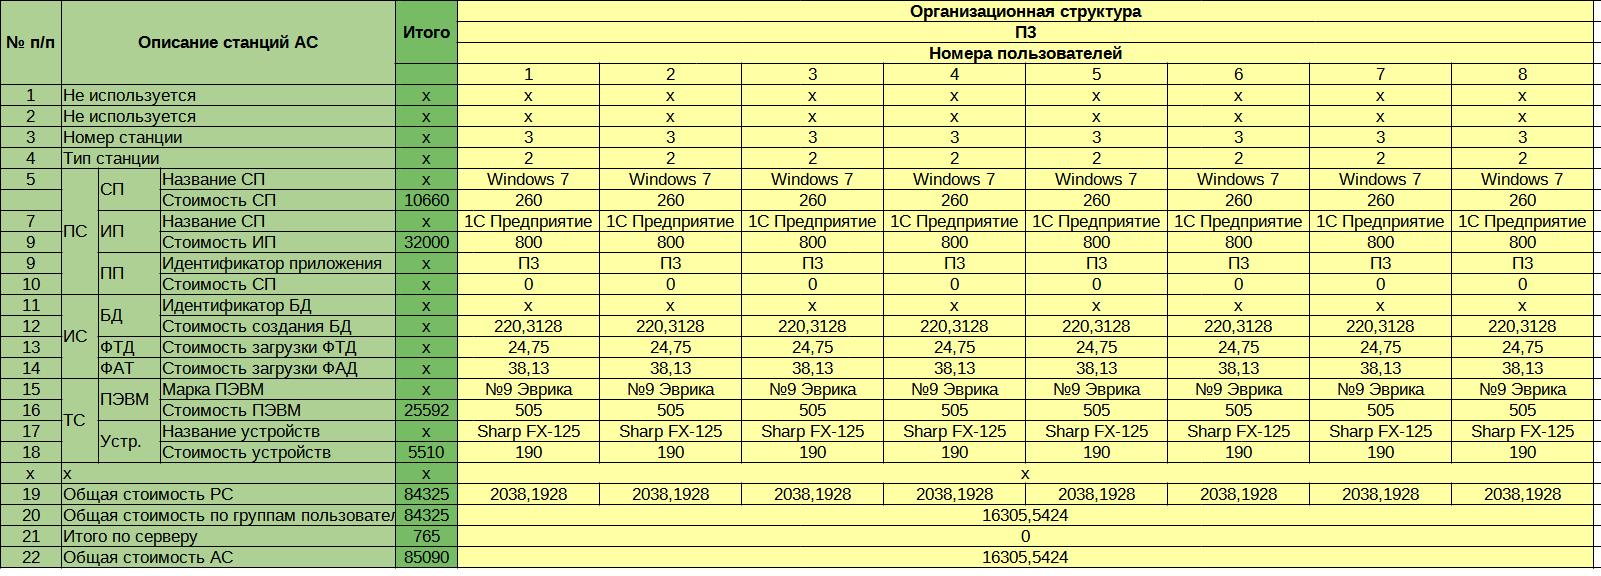
\includegraphics[height=6cm]
            {_docs/КонцепцияАСИЕеКомпонентыП3.jpg}
        \caption{(Таблица 3.1) Концепция АС и её компоненты}
    \end{figure}

    \begin{figure}[!hp]
        \centering
        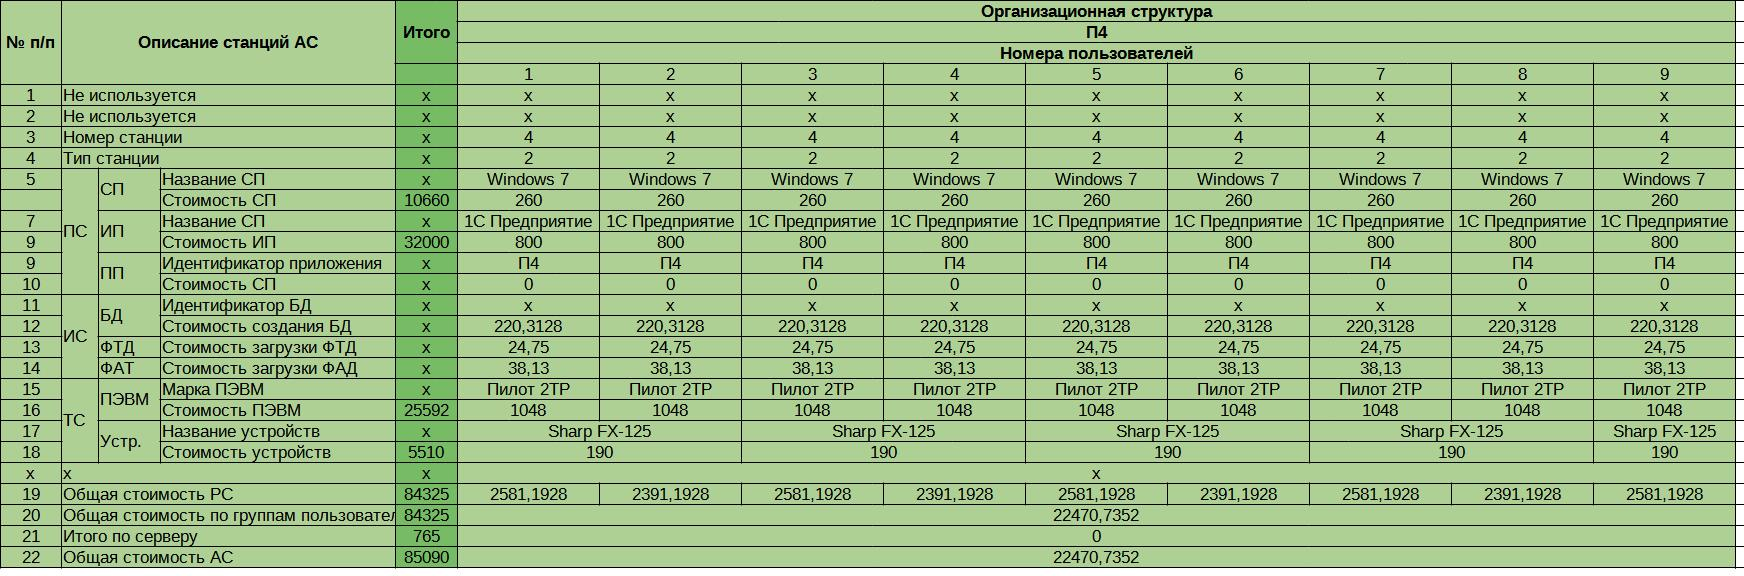
\includegraphics[height=6cm]
            {_docs/КонцепцияАСИЕеКомпонентыП4.jpg}
        \caption{(Таблица 3.1) Концепция АС и её компоненты}
    \end{figure}

    \begin{figure}[!hp]
        \centering
        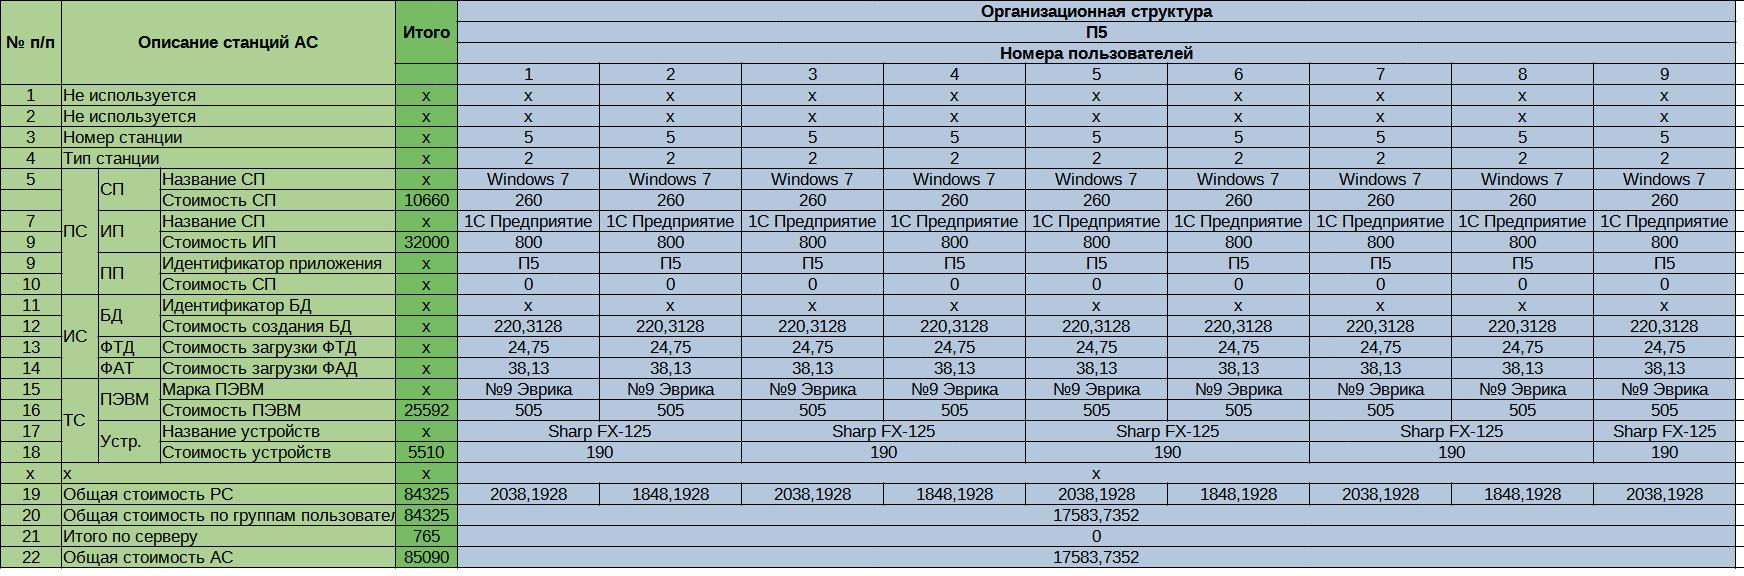
\includegraphics[height=6cm]
            {_docs/КонцепцияАСИЕеКомпонентыП5.jpg}
        \caption{(Таблица 3.1) Концепция АС и её компоненты}
    \end{figure}

    \begin{figure}[!hp]
        \centering
        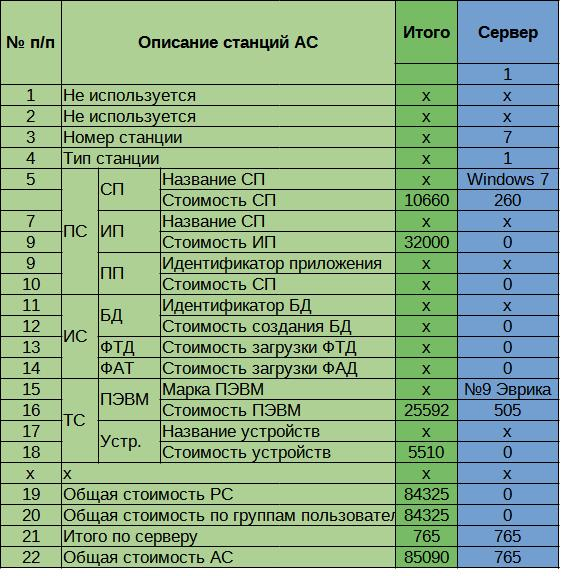
\includegraphics[height=6cm]
            {_docs/КонцепцияАСИЕеКомпонентыСС1.jpg}
        \caption{(Таблица 3.1) Концепция АС и её компоненты}
    \end{figure}
    
    \newpage

    \paragraph{5. Разработка концепции Пс и оценка ее компонент} \hspace{0pt}

    \textbf{Концепция программной системы} АС представляет собой совокупность программных средств в виде системных,
    инструментальных и прикладных программ,
    которые обеспечивают управление функциони­рованием ИС и автоматизируют деятельность пользователей и ЭП. 
    
    \textbf{Системные программы} (СП) - это операционные системы, утилиты и т.д.,
    которые обес­печивают орга­низацию вычислительного процесса и управление устройствами в рамках СС и РС АСОИ на основе ЛВС.
    Пример­ный пе­речень этих программ приведен в табл. Б.3. 
    
    \textbf{Инструментальные программы} (ИП) - это программы, которые используются для реали­зации приклад­ных программ
    (языки программирования, системы управления ба­зами данных и дру­гие),
    а также дру­гие инст­рументальные средства для автоматизации работы пользователей и ЭП ИС.
    Пример­ный пе­ре­чень этих программ приве­ден в табл. Б.3.
    
    \textbf{Прикладные программы} (ПП) - это программы, автоматизирующие деятельность пользователей и ЭП.
    Отдельная задача пользователей или ЭП реализуется в виде отдельной ПП.
    Для пользователей перечень задач и их характе­ристики приведены в табл. Г.2, а для ЭП студент разрабатывает самостоя­тельно.
    
    \textbf{Приложение} - это совокупность прикладных программ,
    которые автоматизируют деятельность опреде­ленной группы (класса) пользователей или ЭП.
   
    Разработка и оценка концепции ПС АС  включает решение следующих задач:
    \begin{enumerate}
        \item[1.] Выбор и оценка стоимости приобретения системных и инструментальных программ для АС.
        \item[2.] Разработка функциональных моделей для ЭП.
        \item[3.] Определение и оценка стоимости создания приклад­ных программ для пользователей и ЭП АС.
    \end{enumerate}

    \paragraph{5.1. Исходные требования для разработки концепции ПС АС} \hspace{0pt}
    
    Для решения задачи по разработке и оценке концепции ПС АС используются следующие требования:

    \begin{enumerate}
        \item[1.] Общие требования заказчика к АС (см. файл ОбщТреб «Группа») – используются только те требова­ния,
        которые влияют на разработку ПС АС.
        \item[2.] Каталог системных и инструментальных средств для ИС (см. табл.Б.3).
        \item[3.] Индивидуальные требования к выбору программных средств для ИС (см. табл. Е.1 и табл. Е.2).
        \item[4.] Модели задач пользователей (см. табл. Г.1).
    \end{enumerate}

    \newpage
    \paragraph{5.2. Определение и оценка системных и инструментальных программ} \hspace{0pt}  
    
    Для каждой СС и РС разработчик осуществляет выбор и оценку стоимости необходимых системных и инструментальных программ.
    
    \textbf{Определение СП и ИП для СС и РС АСОИ}. На основе перечисленных выше требований разработчик для каждой СС и РС выбирает перечень необ­ходи­мых СП и ИП для организации функционирования АС на основе ЛВС. Если не­обхо­димые программы отсутст­вуют, то разработчик может их добавить в табл.Б.3 и за­полнить необходимую о них ин­формацию.  
    
    Для каждой отдельной СС (графа «Сервер») и РС (графа «Номера пользователей») ре­зультаты выбора СП (название и стоимость)
    заносятся в таб­лицу 3.1 (строка 5 – список СП, строка 6 – стои­мость СП).    
    
    Для каждой отдельной РС ре­зультаты выбора ИП (название и стоимость) зано­сятся в таб­лицу 3.1
    (строка 7 – список ИП, строка 8 – стои­мость ИП).  
    
    \paragraph{5.3. Разработка функциональных моделей для ЭП} \hspace{0pt}
    
    Разработка функциональной модели для ЭП. Функциональную модель для ЭП разработчик опреде­ляет самостоятельно и включает определение:
        
    \begin{enumerate}
        \item[1.] Количество задач для ЭП должно определено не менее пяти.
        \item[2.] Вариант модели выбирает один из вариантов предложенных на рис.Г.2 или разрабатывает свой.
        \item[3.] Приводит экспертную оценку характеристики для каждой задачи. 
    \end{enumerate}

    \paragraph{5.4. Определение и оценка прикладных программ} \hspace{0pt}

    Оценка стоимости создания отдельной программы определяется по формуле:

    \begin{lstlisting}[language=Formula]
Стоимость программы = (Общее количество строк программы * Средняя дневная зарплата разработчика)
    / Средняя дневная производительность разработчика
\end{lstlisting}

\begin{itemize}
    \item \textbf{Общее количество строк в программе} – определяется из табл. Г.2;
    \item \textbf{Средняя дневная зарплата} – выбирается разработчиком проекта из диапазона  30 – 70 руб.
    \item \textbf{Средняя дневная производительность разработчика} – выбирается  из диапазона  4 – 10 строк.
\end{itemize} 

    Результаты расчета стоимости ПП и приложений представляются в виде табл. 5.1.

    Итоговые результаты оценки стоимости приложений и их названия для каждой группы пользователей и ЭП зано­сятся
    в строки 9 и 10 табл. 3.1.
    Стоимость разработки отдельного приложения приводится в табл. 3.1 только для одного из представителей группы пользователей.

    \begin{figure}[ph!]
        \centering
        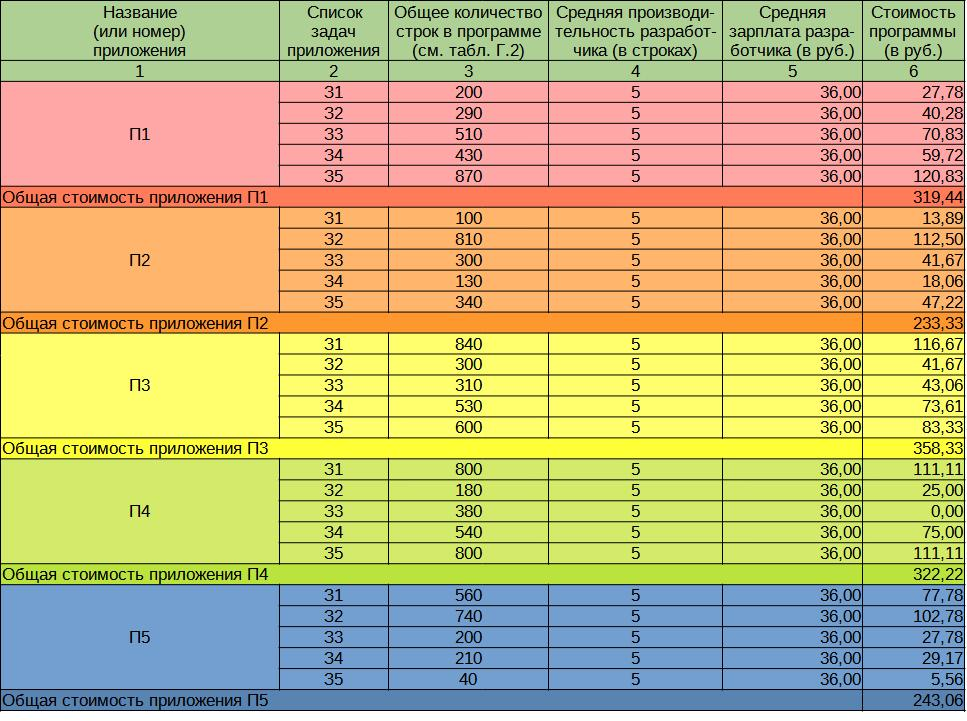
\includegraphics[width=16cm]
            {_docs/ОценкаСтоимостиСозданияПриложений.jpg}
        \caption{(Таблица 5.1) Оценка стоимости и создания изображения}
    \end{figure}

    \newpage

    \paragraph{6. Разработка концепции ис и оценка ее компонент} \hspace{0pt}

    Концепция информационной системы АС представляется совокупностью информационных средств в виде БД и файлов (текущих и архивных документов), расположенных на определенных стан­циях ЛВС и используемых для информационного обеспечения деятельности пользователей ИС.

    Разработка и оценка концепции ИС АСОИ предполагает ре­шение следую­щих задач:
    \begin{enumerate}
        \item[1.] Определение и оценка стоимости создания БД ИС.
        \item[2.] Определение и оценка стоимости загрузки файлов текущих документов (ФТД) в БД ИС.
        \item[3.] Определение и оценка стоимости загрузки файлов архивных документов (ФАТ) в БД ИС.
    \end{enumerate}

    \paragraph{6.1. Исходные требования для разработки концепции ИС АС} \hspace{0pt}

    Для решения задач по разработке и оценке ИС АСОИ используются следующие требования:
    
    \begin{enumerate}
        \item[1.] Общие требования заказчика к АСОИ (см. файл ОбщТреб«Группа»).
        \item[2.] Информационная модель ОА (см. табл. Д.1).
    \end{enumerate}

    \paragraph{6.2. Определение и оценка баз данных} \hspace{0pt}

    \textbf{Оценка стоимости баз данных}.
    Предпологается, что БД в АСОИ одна и является централизованной,
    т.е. доступна для применения всеми пользователями АСОИ.
    Размещается БД на СС АСОИ.
    При необходимости разработчик может предусмотреть несколько БД
    (их расчёт и размещение определяет разработчик).
    Для оценки стоимости создания БД АСОИ используется следующая формула:

    \begin{lstlisting}[language=Formula]
        Стоимость создания БД = (2.94
            + 0.032 * Общее количество атрибутов
            + 2.9 * Общее количество первичных ключей
            + 2.62 * Общее количество внешних ключей
        ) * Дневная зарплата разработчика
\end{lstlisting}
 
    \begin{itemize}
        \item \textbf{Общее количество атрибутов в БД} - определяется из табл. Д.1
        \item \textbf{Общее количество первичных ключей в БД} - определяется из табл. Д.1
        \item \textbf{Общее количество внешних ключей в БД} - определяется из табл. Д.1
        \item \textbf{Дневная зарплата разработчика} - определяет разработчик (диапазон 30-50 руб.)
    \end{itemize}

    \begin{lstlisting}[language=MyFormula]
        Стоимость создания БД = (2.94
            + 0.032 * 320
            + 2.9 * 80
            + 2.62 * 140
        ) * 36 = (2.94 + 10.24 + 232 + 366.8) * 0.36 =
        = 611.98 + 0.36 = 220.3128 ~ 220.31
\end{lstlisting}

    Результаты расчёта представлены в тексте ЛБ и КП и заносятся в табл. 3.1 в строку 12 (графа <<Сервер>>).

    \paragraph{6.3. Определение и оценка текущих и архивных файлов} \hspace{0pt}

    \textbf{Оценка стоимость загрузки файлов в БД АСОИ} определяется по формуле:

    \begin{lstlisting}[language=Formula]
Стоимость загрузки файлов в БД = Объем данных для загрузки в БД * Средняя дневная зарплата
    / Объем вводимых данных за день
\end{lstlisting}

    \begin{itemize}
        \item \textbf{Объём данных для загрузки в БД} - определяется по формуле представленнной далее
        \item \textbf{Средняя дневная зарплата} - определяется разработчиком (диапазон 20 - 30 руб)
        \item \textbf{Объём вводимых данных за день} - определяет разработчик (диапазон 4-8 тыс. символов)
    \end{itemize}    

    Стоимость загрузки определяется отдельно для ФТД и ФАТ.

    Объем данных для загрузки определяется по формуле:

    \begin{lstlisting}[language=Formula]
Объём данных для загрузки = Количество документов * Средний объем документов
    * Среднее количество документов
\end{lstlisting}

    \begin{itemize}
        \item перечисленные в формуле атрибуты определяются из табл. Д.1.
    \end{itemize} 

    Результаты расчёта стоимости загрузки ФТД и ФАТ приводятся в тексте ЛБ и КП и заносятся в табл. 3.1
    (строки 13 и 14 - графа <<Сервер>>).
    
    \begin{lstlisting}[language=MyFormula]
Объём данных для загрузки (ФТД) = 20 * 2.2 * 150 = 6600
Объём данных для загрузки (ФАД) = 80 * 3.1 * 41 = 10 168
\end{lstlisting}

\begin{lstlisting}[language=MyFormula]
Стоимость загрузки файлов в БД (ФТД) = 6600 * 30 / 8000 = 24.75
Стоимость загрузки файлов в БД (ФАД) = 10 168 * 30 / 8000 = 38.13
\end{lstlisting}

    \newpage

    \begin{figure}[h!]
        \centering
        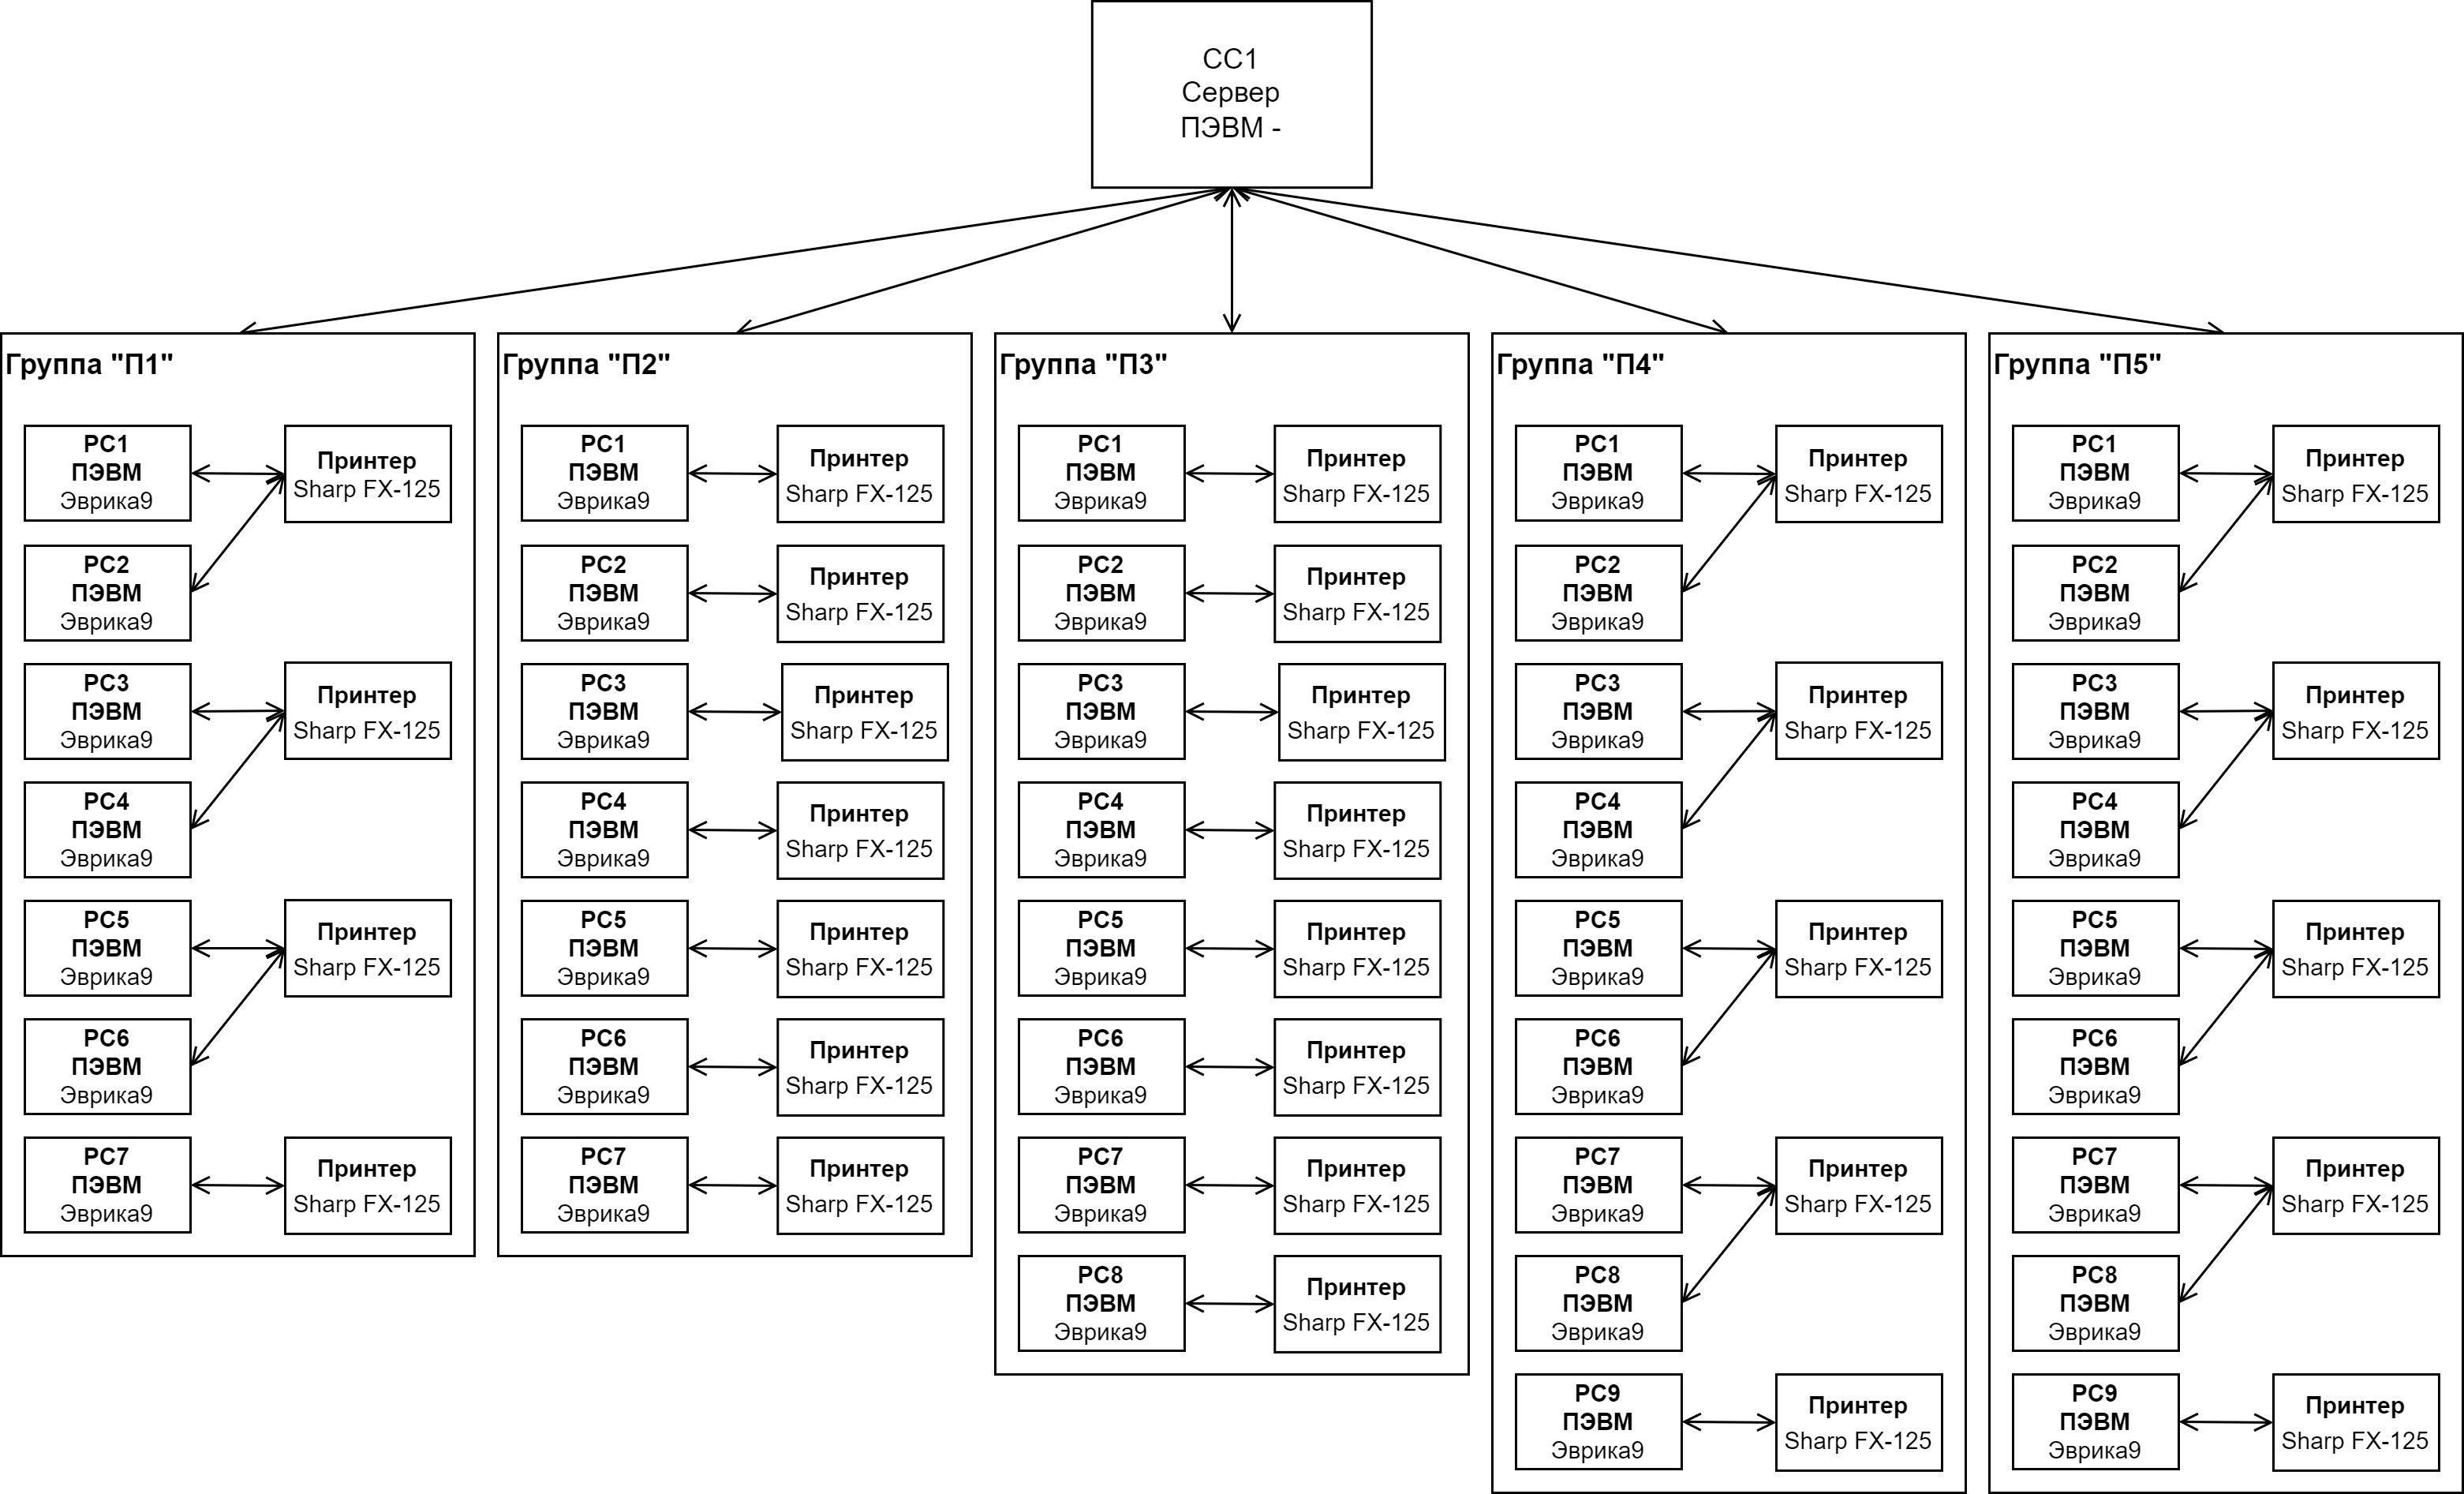
\includegraphics[width=16cm]
            {_docs/ЛогическаяСтруктураТСАСОИ.png}
        \caption{(Рисунок 7.1) Логическая структура ТС АСОИ}
    \end{figure}

%     \paragraph{} \textbf{Исходный код}: 

%     \lstinputlisting[language=c]{src/HelloWorld.c}

%     \begin{lstlisting}[caption=Вывод в консоль]
%  Hello, World!
% \end{lstlisting}

%     \paragraph{} \textbf{Вывод}: создали отчёт, используя \LaTeX.

    % % = = = = = = = =
    % % \newpage
    % % \addcontentsline{toc}{section}{Список использованных источников}
    % \section*{Список использованных источников}
    % \begin{enumerate}
    %     \item[1.] eskdx.pdf [Электронный ресурс]
    %     - Режим доступа: \url{http://tug.ctan.org/macros/latex/contrib/eskdx/manual/eskdx.pdf}.
    %     Дата~доступа:~20.02.2022.
    %     \item[2.] Опции пакета hyperref [Электронный ресурс]
    %     - Режим доступа: \url{https://grammarware.net/text/syutkin/hyperref_options.pdf}.
    %     Дата~доступа:~20.02.2022.
    % \end{enumerate}
    % \newpage
\end{document}
